%% safe2026-v3.tex
%% SAFE 2026 -- Sustainable Accounting, Finance and Economics International Conference.
%% v3: the flood-screening work re-angled for a finance/economics audience.
%% Target theme: "Climate Risk, Regulation and Financial Stability"
%%   (climate-related financial risks and risk management; environmental risk
%%    disclosure and compliance; financial-stability / systemic trade risk).
%% Single-column article format (swap to the SAFE2026 template when published).
%% Figures are shared with the v2 paper (./figures/, generated by
%% scripts/render_v2_fig{1..4}_*.py). Compile: pdflatex safe2026-v3.tex (twice).

\documentclass[11pt,a4paper]{article}

\usepackage[margin=1in]{geometry}
\usepackage{amsmath,amssymb}
\usepackage{graphicx}
\usepackage{booktabs}
\usepackage{enumitem}
\usepackage{textcomp}
\usepackage[T1]{fontenc}
\usepackage[utf8]{inputenc}
\usepackage{cite}
\usepackage{caption}
\usepackage[hidelinks]{hyperref}
\captionsetup{font=small,labelfont=bf}
\graphicspath{{figures/}}

\title{\textbf{Closing the Physical Climate-Risk Information Gap:\\
An Open, Validated Multi-Hazard Flood Screen for Climate-Related\\
Financial Risk Management in Under-Resourced Southeast Asian Cities and Ports}}

\author{Daniel Phang\thanks{Nanyang Technological University, Singapore. \texttt{phan0038@e.ntu.edu.sg}}
\and Tze-Houng Lee\thanks{National University of Singapore, Singapore. \texttt{thlee@nus.edu.sg}}}
\date{}
% For double-blind review, replace the \author block with: \author{}

\begin{document}
\maketitle

\begin{abstract}
\noindent Physical climate risk is increasingly material to financial decisions --- asset valuation, insurance, credit allocation, infrastructure finance, and the deployment of adaptation capital --- yet the firms, municipalities, and supervisors most exposed to it in Southeast Asia are precisely those least able to obtain usable hazard information. The only comparable-resolution (30\,m) three-hazard regional flood model is commercial and closed, and its free tier excludes the major ASEAN megacities and the ports that anchor regional trade; bespoke engineering studies are rarely published openly; and open global products are an order of magnitude coarser and omit the pluvial (rain-driven) hazard that dominates urban flooding here. The result is an information market failure: exposure that materially affects asset values and financial stability cannot be screened, priced, or disclosed by the agencies that most need to. We present an open-source, open-data pipeline that produces design-event coastal, fluvial, and pluvial flood-depth maps at 30\,m for Singapore, Kuala Lumpur, Bangkok, and Jakarta under four climate combinations (SSP2-4.5/SSP5-8.5 $\times$ 2050/2100), with the pluvial hazard anchored to each national meteorological service's published Intensity--Duration--Frequency (IDF) standard. We make the resulting risk surface \emph{trustworthy}, not merely reproducible: a pre-defined, model-blind location-skill gate yields statistically significant discriminative skill in all four cities (one of four also clearing a stricter joint sensitivity/specificity bar), and a bathtub coastal over-prediction of 1.7--25$\times$ at the 100-year return period is structurally corrected by a local-inertia solver. Framed as open decision-support infrastructure for climate-related financial risk management, scenario-based disclosure, and forward-looking adaptation investment, the release is offered as a public good for the agencies that commercial models exclude.

\medskip
\noindent\textbf{Keywords:} climate-related financial risk, physical risk, environmental risk disclosure, financial stability, adaptation finance, open data, Southeast Asia.\\
\noindent\textbf{Target theme:} Climate Risk, Regulation and Financial Stability.
\end{abstract}

\section{Introduction}
Climate change has become a first-order concern for financial stability: a hazard distribution that shifts warmer raises the frequency of damaging extremes far faster than it raises the mean, so risk priced on the historical record is systematically under-priced~\cite{carney2015,ngfs2021}. For physical assets the exposure is concrete. Southeast Asia contains six of the ten cities globally most exposed to coastal flooding by 2100 under high-emission scenarios, roughly 750~million people, and about a fifth of regional GDP on flood-exposed land~\cite{adb2022}. The stressors compound: AR6 median sea-level rise (SLR) under SSP5-8.5 by 2100 ranges from $+0.62$\,m (Singapore) to $+1.62$\,m (Bangkok)~\cite{ar6}; tropical convective rainfall intensifies at or above the Clausius--Clapeyron rate~\cite{lenderink2017}; and several megacities subside at 1--25\,cm\,yr$^{-1}$~\cite{chaussard2013,abidin2011,phienwej2006}. The 2011 Thailand megaflood, the 2020 Jakarta monsoon floods, and the 2021 Kuala Lumpur flash floods are recent reminders that the exposure is multi-hazard (coastal, fluvial, and pluvial) and concurrent~\cite{hallegatte2013,tellman2021}.

These same cities anchor the financial and trade system. Maritime transport carries over 80\% of world trade by volume, and ASEAN hosts both top-tier ports (Singapore, Port Klang, Tanjung Priok, Laem Chabang) and the Strait of Malacca chokepoint. Ports are critical, long-lived infrastructure with a multi-year planning phase and a 50-year-plus useful life, so an asset financed today operates well into the zone of large climate uncertainty~\cite{hanson2020}. This is precisely the ``tragedy of the horizon'' that makes climate risk hard to price: the costs fall beyond the planning and reporting cycle of most actors, so they are under-weighted until they crystallise~\cite{carney2015}. Present-day multi-hazard damage to global port infrastructure already carries an expected value at risk of about \$7.6~billion per year (range \$4.0--17.4~billion), with roughly 80\% of ports exposed to flooding~\cite{verschuur2023}. First-order hazard screening is the cheapest input to the resulting trillion-dollar adaptation and disclosure question, yet it is exactly what under-resourced ASEAN municipalities, port authorities, and their financiers cannot obtain.

\textbf{An information market failure.} Disclosure and supervisory frameworks now require firms to assess physical climate risk under forward-looking scenarios~\cite{tcfd2017,issb2023}, and supervisors increasingly run physical-risk stress scenarios~\cite{ngfs2021}. All of these presuppose a usable hazard surface. Existing tools fall into three categories, none of which simultaneously offers high resolution, multi-hazard scope, open code, open data, and per-country calibration (Table~\ref{tab:landscape}). The only 30\,m three-hazard global model is commercial~\cite{wing2024}, and its free tier excludes the major ASEAN megacities. Bespoke municipal studies are typically proprietary and seldom published in a form others can reproduce. Open global alternatives are an order of magnitude coarser ($\sim$10\,km) and lack the pluvial layer that drives most urban flood damage in the region~\cite{hofste2019,ward2020,sutanudjaja2018}. The result is an equity gap with a financial edge: the institutions that most need to price and disclose physical risk --- in exactly the cities the commercial free tier omits --- cannot, so the risk is mispriced, under-insured, or ignored.

This paper addresses that gap. We present an open-source, open-data, per-country-calibrated 30\,m multi-hazard flood pipeline and atlas for four ASEAN cities, validate that it locates real floods, and frame it as decision-support infrastructure for climate-related financial risk: in a ``new climate era,'' management, disclosure, and capital allocation must screen on return periods and explicit climate scenarios rather than extrapolate a stationary past.

\textbf{Academic contributions.} The released atlas is a resource contribution: to our knowledge it is the first open, reproducible, per-country-calibrated 30\,m three-hazard flood product for the region. Its scholarly value, however, lies in four findings that are transferable beyond our four-city release:
\begin{enumerate}[leftmargin=*,itemsep=2pt,topsep=3pt]
\item \emph{A pre-registered, model-blind location-skill protocol for open flood screening.} A frozen register of documented-flooded and documented-dry localities is scored by the true-skill statistic with a bootstrap confidence interval, under an explicit separation between significant skill and a stricter PASS bar and a dry-control discipline that forbids retuning. We show the protocol transfers across four cities with no engine changes, turning ``reproducible'' into the stronger, testable claim ``demonstrably skilful'' --- the property a disclosure- or supervision-grade risk surface actually needs.
\item \emph{A quantified characterisation and structural correction of bathtub bias in 30\,m open coastal screening.} The connectivity (bathtub) solver that is the default in open tools over-predicts inundation at the 100-year return period (RP100) by 1.7--25$\times$; we show this is a solver-architecture artifact, removed by a local-inertia shallow-water solver (Bangkok 12.5$\times{\rightarrow}$1$\times$), rather than a 30\,m data-resolution limit. Uncorrected, this bias would inflate any value-at-risk computed from open screens on deltaic terrain.
\item \emph{Per-country Intensity--Duration--Frequency (IDF) anchoring to close the tropical-convective pluvial deficit.} We quantify a 28--62\% shortfall of global-synthetic design rainfall against four national IDF standards and give a two-anchor recipe that eliminates it, the single most important in-region calibration for the pluvial layer that global products omit.
\item \emph{A main-stem-HAND referencing rule, with its failure boundary.} HAND must be referenced to the trunk channel the modelled discharge represents (a 180\,km\textsuperscript{2} accumulation trunk) rather than a channel-initiation threshold or the full OSM network; we validate this against the skill gate and delimit where single-stage HAND fails (flat deltas fed by an out-of-domain mega-river).
\end{enumerate}
Each is stated as a finding others can reuse independently of our specific release; the conceptual contribution, reframing screening as forward-looking, distribution-aware decision support (Sec.~\ref{sec:context}), ties them to the financial decisions they serve.

\begin{table}[t]
\centering
\caption{Comparator landscape for ASEAN-relevant flood-screening tools.}
\label{tab:landscape}
\small
\begin{tabular}{@{}lcccc@{}}
\toprule
Tool                                    & Res.           & Hazards        & Open code/data   & Per-country IDF \\
\midrule
\textbf{This work}                      & \textbf{30\,m} & \textbf{C+F+P} & \textbf{Yes/Yes} & \textbf{Yes (4 svc.)} \\
Fathom 3.0~\cite{wing2024}              & 30\,m          & C+F+P          & No/No            & Global synth.$^{\dag}$ \\
Aqueduct 4.0~\cite{hofste2019,ward2020} & $\sim$10\,km   & C+F            & Method/Yes       & None \\
GLOFRIS~\cite{sutanudjaja2018}          & $\sim$10\,km   & F\,(+C)        & Yes/Yes          & None \\
City studies                            & High           & Various        & No/No            & Per-city \\
\bottomrule
\end{tabular}

\vspace{3pt}
{\footnotesize $^{\dag}$Fathom's free tranche (accessed and verified 2025) is restricted to selected developing countries and excludes the major ASEAN megacities covered here. The comparison axis is openness and access rather than accuracy: Fathom is bare-earth and engineering-validated; we claim open reproducibility for omitted cities rather than terrain or skill parity. C\,=\,coastal, F\,=\,fluvial, P\,=\,pluvial.}
\end{table}

\section{Decision Context: Why Climate-Risk Screening Must Be Forward-Looking}
\label{sec:context}
Infrastructure optimised for the twentieth-century climate now faces conditions outside its design envelope, and the financial consequence follows from a property of shifting distributions rather than any single forecast: as a hazard distribution shifts warmer, the frequency of extremes grows much faster than the mean. Fig.~\ref{fig:distshift} makes this concrete with a schematic Gaussian shift: a mean shift of one standard deviation raises the probability of exceeding a ``$+2\sigma$'' threshold from 2.3\% to 15.9\%, roughly a 7$\times$ jump that turns a 44-year event into a 6-year event, even though the average moved only modestly~\cite{patel2024}. (The 2.3\%/15.9\% values are the normal-distribution tail beyond $2\sigma$ and $1\sigma$; the figure illustrates the mechanism rather than a specific IDF curve.) A balance sheet, an insurer, or a supervisor that prices flood risk by extrapolating the historical record therefore systematically under-prices the tail. The corrective, and the basis of every credible climate stress test, is to screen on return periods and explicit climate scenarios~\cite{ngfs2021} --- which is exactly the surface our atlas provides.

The decision relevance is sharpened by the long life of the assets at risk (Fig.~\ref{fig:assetlife}). A port entering planning today is completed in the mid-2030s and operates into the 2080s, by which point SSP-pathway divergence is wide: median ASEAN SLR by 2100 spans $+0.62$ to $+1.62$\,m, with larger high-end ranges. Two realities frame how the screen will be used. First, adaptation lags mitigation: among the largest global ports, 89\% (31/35) have mitigation plans but only 66\% (23/35) have adaptation plans~\cite{jpm_seachange}, a gap that is itself a disclosed-risk signal. Second, hard remediation is slow and costly: the U.S. Coastal Texas (``Ike Dike'') barrier is projected at \$57~billion over a 20-year build~\cite{usace_coastaltexas}, so a cheap, open, comparable screen is the rational first move before committing capital. Global port investment to keep pace with SLR and trade growth is estimated at \$223--768~billion by 2050~\cite{hanson2020}; deciding \emph{where} that capital goes begins with screening.

\begin{figure}[t]
\centering
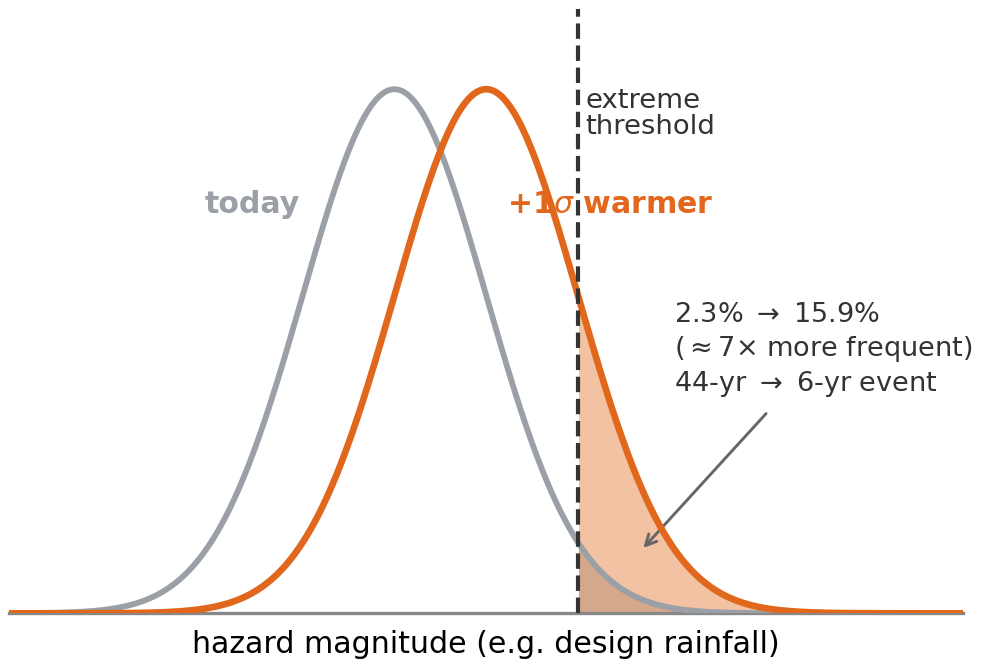
\includegraphics[width=0.62\textwidth]{fig1_distshift.png}
\caption{Climate ``math'' for screening. A schematic mean shift of one standard deviation produces a large, non-linear increase in threshold-exceedance frequency (here ${\approx}7\times$). Risk priced by static extrapolation of the historical record under-prices the tail; return-period, scenario-conditioned screening does not.}
\label{fig:distshift}
\end{figure}

\begin{figure}[t]
\centering
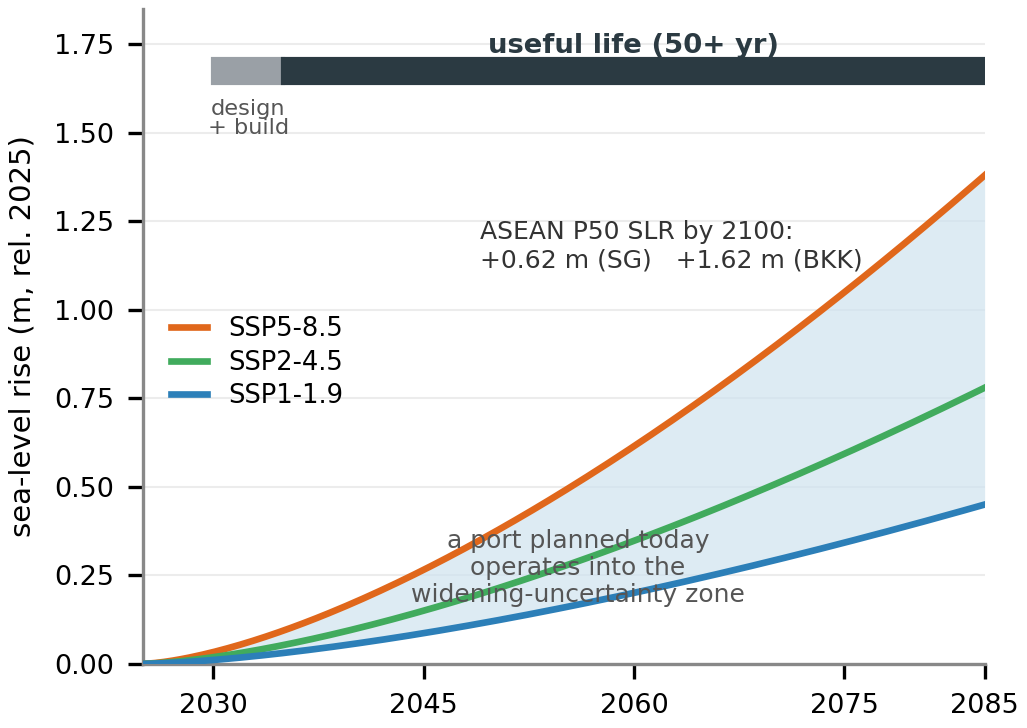
\includegraphics[width=0.66\textwidth]{fig2_assetlife.png}
\caption{Asset life versus scenario uncertainty --- the ``tragedy of the horizon'' made visual. A port planned today operates through the 2080s, deep inside the widening SLR fan (SSP1-1.9/SSP2-4.5/SSP5-8.5; ASEAN P50 endpoints $+0.62$\,m SG, $+1.62$\,m BKK from~\cite{ar6}). The screen exists to make that fan, across scenario and horizon, legible before capital is committed.}
\label{fig:assetlife}
\end{figure}

\section{The Open Multi-Hazard Pipeline}
A per-city configuration drives a single orchestration script (Fig.~\ref{fig:pipeline}). Every input is free and most require no registration: the Copernicus GLO-30 DEM, ERA5-Land precipitation~\cite{era5land}, UHSLC tide gauges, GloFAS~v4 discharge reanalysis~\cite{glofas}, IPCC AR6 SLR projections~\cite{ar6}, ESA WorldCover 2021~\cite{worldcover}, and OpenStreetMap waterways. The implementation is pure Python on the scientific stack; no external binaries or licensed data are required, which is what makes third-party rebuild from scratch possible --- the precondition for an audit-grade risk input.

\textbf{Per-country IDF anchoring.} The most important in-region calibration is the pluvial design rainfall. Global synthetic statistics under-represent tropical-convective extremes. We quantify the shortfall per service as the relative deficit against the national IDF curve at matched duration and return period; across the four services (PUB, JPS-MSMA, TMD-RID, BMKG) it spans 28--62\%. As an illustrative single cell, a national 6-hour 100-year design depth of $\sim$250\,mm against a global-synthetic $\sim$155\,mm is a 38\% shortfall, a gap that propagates directly into ponding depth and hence into any damage or value-at-risk estimate built on it. We fit a two-anchor Gumbel distribution to each country's published standard; two (return period, depth) anchors exactly determine Gumbel's two parameters, so this is exact determination rather than a regression fit, anchored to the published national standard.

\textbf{Three hazards.} \emph{Coastal:} a GEV fit to UHSLC annual-maximum storm-surge residuals (T\_TIDE-detided~\cite{ttide}), consistent with global surge reanalyses~\cite{muis2016,muis2020}, plus the AR6 SLR delta, routed by a local-inertia shallow-water solver~\cite{bates2010}; a connectivity bathtub solver is retained only as a fallback. \emph{Fluvial:} the GloFAS design discharge is converted to a design stage and mapped via Height Above Nearest Drainage (HAND)~\cite{nobre2011,renno2008} referenced to the main-stem trunk the modelled discharge represents (for Kuala Lumpur, the $\geq 180$\,km\textsuperscript{2} accumulation trunk) rather than a channel-initiation threshold or raw OSM network. \emph{Pluvial:} the IDF excess is routed by a catchment-routed fill-and-spill cascade~\cite{barnes2021} (depressions resolved by a Planchon--Darboux fill~\cite{planchon2002}) with a per-cell runoff coefficient from WorldCover. The three depth rasters are composited by per-pixel maximum. All hazards are produced for SSP2-4.5 and SSP5-8.5 at 2050 and 2100 on a subsidence-corrected DEM, with the subsidence component reported separately for sensitivity rather than buried in the forcing.

\begin{figure}[t]
\centering
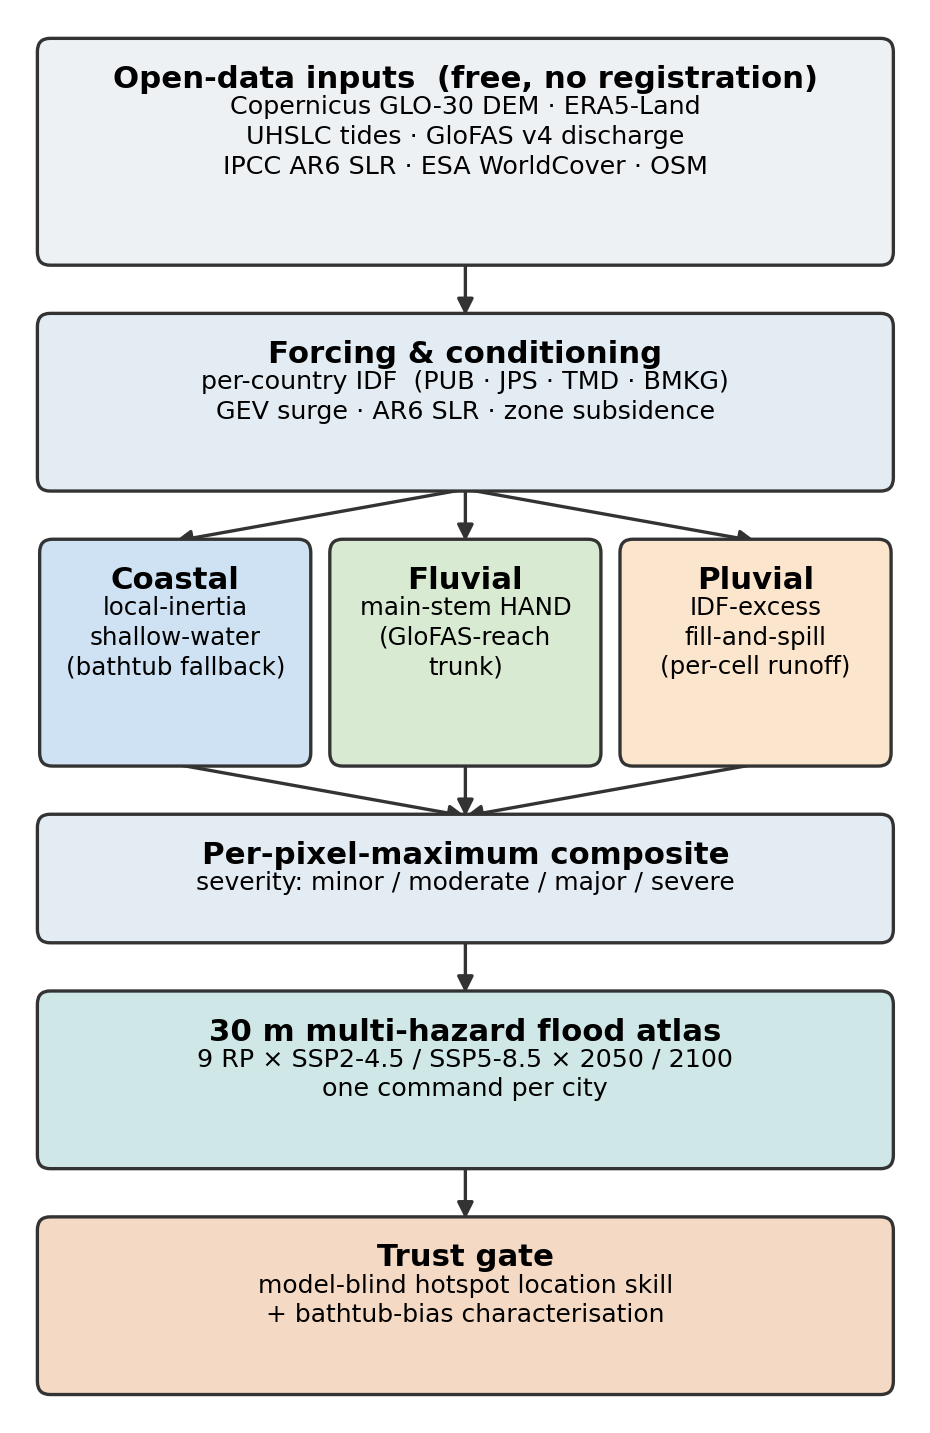
\includegraphics[width=0.5\textwidth]{fig3_pipeline.png}
\caption{Pipeline data flow: free open-data inputs $\rightarrow$ forcing \& conditioning $\rightarrow$ per-hazard solvers (inertial coastal, main-stem-HAND fluvial, fill-and-spill pluvial) $\rightarrow$ per-pixel-maximum composite and severity classification $\rightarrow$ trust gate.}
\label{fig:pipeline}
\end{figure}

\section{The Open Flood Atlas: a Risk Surface}
At the canonical RP100\,/\,SSP5-8.5\,/\,2100 combination the atlas shows the expected physical contrast between cities (Table~\ref{tab:extent}): low-lying Bangkok is coastal-dominated under the raw solver, Jakarta fluvial/pluvial, and inland Kuala Lumpur pluvial. The headline combined extent is sensitive to the coastal solver: the bathtub layer over-predicts (Sec.~\ref{sec:validation}), so we present coastal extents both ways, and substituting the inertial layer collapses Bangkok's combined extent from 3{,}598 to ${\approx}900$\,km\textsuperscript{2}. For a risk user the practical rule is that exposure and any value-at-risk derived from it must be read off the corrected (inertial) column; the bathtub column is shown only to expose the correction.

\begin{table}[t]
\centering
\caption{Combined flood extent at RP100, SSP5-8.5\,/\,2100 (km\textsuperscript{2}). Coastal shown as bathtub~$\rightarrow$~inertial.}
\label{tab:extent}
\small
\begin{tabular}{@{}lccrrl@{}}
\toprule
City         & Coast.                                    & Fluv.                  & Pluv. & Comb.$^{\ddag}$ & Dominant \\
\midrule
Singapore    & 67\,$\rightarrow$\,48$^{\S}$               & 112$^{*}$              & 19    & 184             & canal+coast \\
Kuala Lumpur & 0\,$\rightarrow$\,0                        & 126                    & 268   & 362             & pluvial \\
Bangkok      & 3{,}546\,$\rightarrow$\,\textbf{283}       & 788                    & 433   & ${\approx}$900  & fluvial \\
Jakarta      & 159\,$\rightarrow$\,112                    & 389                    & 169   & 560             & fluv.+pluv. \\
\bottomrule
\end{tabular}

\vspace{3pt}
{\footnotesize $^{\ddag}$Combined uses the inertial coastal layer for every row; Bangkok combined is the headline correction (bathtub combined was 3{,}598). $^{\S}$Singapore's documented present-day coastal baseline is near zero, so its residual ratio is an artefact (Sec.~\ref{sec:validation}). $^{*}$Singapore's ``fluvial'' layer is PUB primary canal-overflow under long-duration design rainfall rather than natural-river flooding.}
\end{table}

\textbf{The mitigation delta, corrected.} The cleanest single number for an adaptation planner or an insurer pricing avoided loss is the mitigation delta, the flooded area avoided by meeting the lower-emissions pathway. On the bathtub layer the avoided Bangkok coastal RP100 land (SSP2-4.5 vs SSP5-8.5 at 2100) is $-133$\,km\textsuperscript{2}. Such deltas are sometimes assumed robust to absolute bias, but that holds only for additive offsets; the bathtub bias is multiplicative ($\sim$12.5$\times$ for Bangkok), so computed on the corrected inertial layer the avoided area is ${\approx}11$\,km\textsuperscript{2}, an order of magnitude smaller. The sign and policy direction are robust; the magnitude carries the residual bias and must be read off the inertial layer. A risk metric built on the uncorrected delta would over-state the value of mitigation tenfold.

\section{Validation and Trustworthiness}
\label{sec:validation}
A risk surface is only useful if it can be trusted to flood where flooding actually occurs --- the difference between a defensible disclosure and a liability. We test this with a pre-defined, model-blind documented-hotspot location-skill gate. For each city we freeze, before consulting any model output, a register of localities with documented flooding (positives) and localities documented to have stayed dry (controls), each geocoded and DEM-verified. The combined present-day wet mask (pluvial $\vee$ fluvial $\vee$ coastal, $\geq 0.10$\,m, within a 50\,m hit radius) is scored at the event-matched RP100, reporting hit-rate (HR; sensitivity), correct-reject-rate (CRR; specificity), and the true-skill statistic (TSS $=$ HR $+$ CRR $- 1$) with a BCa bootstrap 95\% confidence interval (10{,}000 resamples); the $2\times2$ association is corroborated by Fisher's exact test.

\begin{table}[t]
\centering
\caption{Documented-hotspot gate (present-day, RP100, $\geq 0.10$\,m, 50\,m). PASS $=$ HR $\geq 0.70 \wedge$ CRR $\geq 0.70 \wedge$ TSS CI $>0$.}
\label{tab:gate}
\small
\begin{tabular}{@{}lccccl@{}}
\toprule
City         & pos/dry & HR   & CRR  & TSS [95\% CI]              & verdict \\
\midrule
Kuala Lumpur & 17/7    & 0.76 & 0.86 & \textbf{0.62} [0.25, 0.88] & \textbf{PASS} \\
Singapore    & 38/20   & 0.82 & 0.65 & \textbf{0.47} [0.21, 0.72] & sig.; CRR$<$.70 \\
Bangkok      & 16/7    & 0.56 & 0.86 & \textbf{0.42} [0.04, 0.75] & sig.; HR$<$.70 \\
Jakarta      & 18/8    & 0.89 & 0.50 & \textbf{0.39} [0.03, 0.75] & sig.; CRR$<$.70 \\
\bottomrule
\end{tabular}

\vspace{3pt}
{\footnotesize Jakarta is reported both ways: before the model-blind reclassification of two record-documented controls (Menteng, Gambir; inundated 2007 and 2013) TSS was 0.16 (no skill); after, 0.39. The reclassification was fixed on flood-record evidence before the first gate run, never to make the gate pass.}
\end{table}

\textbf{Two reported bars.} We distinguish two criteria that are easily conflated. \emph{Significant discriminative skill} is the weaker condition that the TSS confidence interval excludes zero. \emph{PASS} is the stricter, pre-registered bar HR $\geq 0.70$ \emph{and} CRR $\geq 0.70$ \emph{and} TSS CI $>0$. All four cities meet the weaker condition; one (Kuala Lumpur) meets PASS (Table~\ref{tab:gate}). Kuala Lumpur's PASS survives a Bonferroni-adjusted $\alpha = 0.0125$, as does the pooled register. We acknowledge the small registers (24/58/23/26 points): the lower CI bounds of 0.03--0.04 for Bangkok and Jakarta are statistically significant but fragile, and we present them as such. The remaining shortfalls are documented structural limits rather than tuning failures: Bangkok's HR is bounded because the 2011 reference flood was sourced from a catchment whose headwaters lie outside the model domain~\cite{komori2012}, and Jakarta's residual specificity loss is fill-and-spill over-ponding on elevated ground.

\textbf{Bathtub bias is structurally corrected.} A bathtub solver, the default in open screening tools, over-predicts documented present-day coastal inundation by 1.7--25$\times$ at RP100, because 30\,m terrain cannot resolve the sub-pixel road raises, canals, and bunds that protect small present-day events. Replacing it with the local-inertia solver brings the over-prediction to ${\approx}1\times$ (Fig.~\ref{fig:bias}): Bangkok's RP100 coastal extent drops from 3{,}546 to 283\,km\textsuperscript{2} (a 12.5$\times$ reduction). The correction is architectural: Singapore's residual 18$\times$ ratio is an artefact of its near-zero documented baseline rather than a model failure. For a risk user, this is the difference between a credible exposure figure and one inflated by more than an order of magnitude.

\begin{figure}[t]
\centering
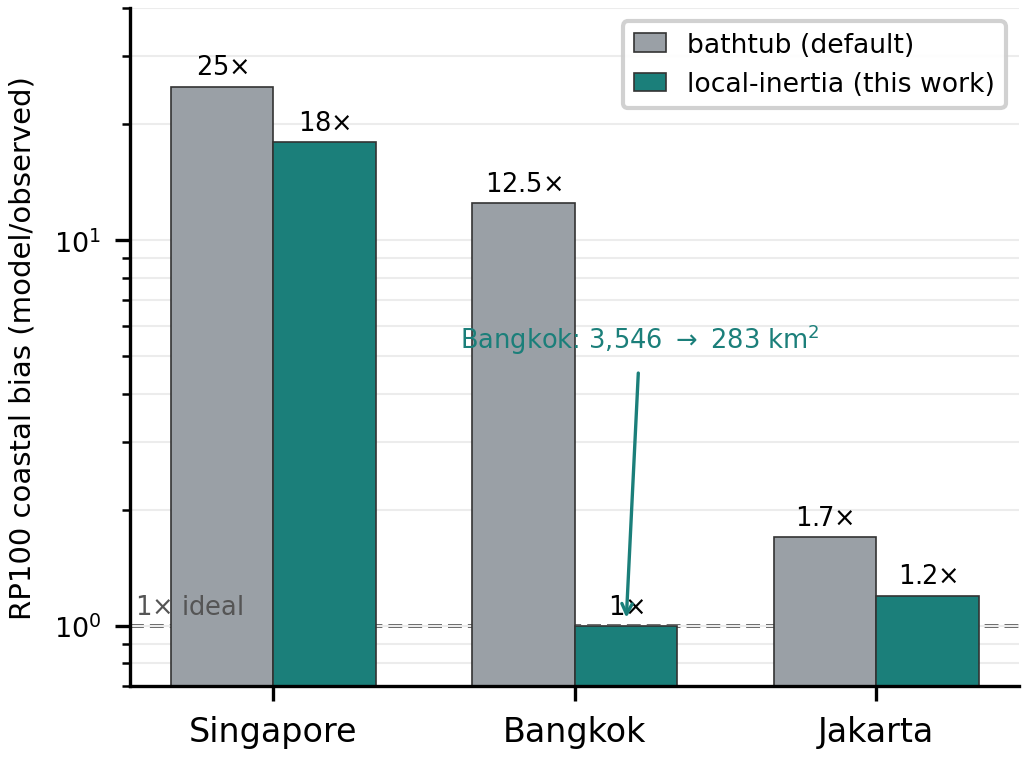
\includegraphics[width=0.6\textwidth]{fig4_bathtub_bias.png}
\caption{Bathtub-bias factor (model/observed) at RP100 by city, with the local-inertia correction (log scale). The 12.5$\times$ Bangkok reduction to ${\approx}1\times$ (3{,}546~$\rightarrow$~283~km\textsuperscript{2}) is the headline; Singapore's residual ${\approx}18\times$ reflects a near-zero documented baseline.}
\label{fig:bias}
\end{figure}

\section{From Risk Screening to Financial Decisions}
The atlas is a decision instrument, and for a finance or economics audience its value tracks three uses. \emph{Risk management and disclosure:} forward-looking physical-risk assessment under explicit scenarios is now a disclosure and supervisory expectation~\cite{tcfd2017,issb2023,ngfs2021}, and an open, validated, scenario-conditioned hazard surface is the missing input for the agencies and firms that cannot license a commercial one --- turning physical-risk disclosure from a procurement question into a software install. \emph{Adaptation capital allocation:} because the same solver and inputs are used for every city and scenario, cross-scenario deltas (read off the corrected layer) isolate the adaptation-relevant signal from absolute bias, letting an agency or financier triage sites before commissioning costly bespoke studies; with global port adaptation alone estimated at \$223--768~billion by 2050~\cite{hanson2020}, even a coarse but unbiased screen has high option value. \emph{Financial-stability and systemic-trade risk:} 80\% of ports face flooding exposure and present-day port damage risk is $\sim$\$7.6~B\,yr$^{-1}$, with 32\% concentrated in cyclone-prone clusters~\cite{verschuur2023}; because ASEAN hosts the Malacca chokepoint, physical risk to these specific assets is not idiosyncratic but systemic to regional trade and supply chains. The cities our atlas covers are exactly the assets a commercial model's free tier omits, so closing the information gap is simultaneously a humanitarian, a market-efficiency, and a financial-stability good.

\section{Impact and Limitations}
The intended use is a public good: open, validated, reproducible hazard maps as decision support for the municipal, port, insurance, and supervisory users that cannot license commercial models. The model is a screening upper bound under three explicit assumptions: no active pumping, no sub-pixel defences resolved by the 30\,m DEM, and per-pixel-maximum (marginal rather than joint-exceedance) composition --- so it informs screening and triage, not asset-level engineering design or final loss settlement. Two findings bound transferability and are reported rather than tuned away: single-stage HAND does not transfer to flat deltas fed by an out-of-domain mega-river (Bangkok, Jakarta)~\cite{komori2012}, which bounds Bangkok's HR; and the pluvial fill-and-spill solver is steady-state and currently heterogeneous across cities, which explains residual specificity loss. Terrain is the dominant residual bias source: the GLO-30 DSM includes buildings and vegetation, which drives the bathtub over-prediction, so migrating to a free bare-earth product (FABDEM) is the named next step. Extending the bias-aware coastal treatment to fully enclosed-sea topologies is the principal prerequisite for broader regional coverage. None of these limits the core financial claim: the surface is an honest, validated, scenario-conditioned screen that did not previously exist openly for these cities.

\section{Conclusion}
Physical climate risk is material to financial stability, but it cannot be priced, disclosed, or adapted to where it cannot be screened. We have shown that an open-source, open-data, per-country-calibrated 30\,m multi-hazard flood atlas for ASEAN cities is feasible, reproducible from free data, and --- by a pre-defined, model-blind location-skill gate --- demonstrably skilful in the four cities tested, with its coastal over-prediction structurally corrected so that every headline number is read off the corrected layer. By targeting exactly the cities and ports that commercial high-resolution models exclude, and by framing the output as forward-looking decision-support infrastructure for climate-related financial risk management, disclosure, and adaptation investment under deep uncertainty, the release is offered as a public good for closing a physical-risk information gap with humanitarian, market-efficiency, and financial-stability consequences.

\section*{Reproducibility}
Code, per-city configuration, and the frozen validation registers are released openly, enabling third-party rebuild of every result from free data. (For double-blind review, an anonymised mirror is provided and the de-anonymised repository on acceptance.)

\begin{thebibliography}{00}
\bibitem{carney2015} M. Carney, ``Breaking the tragedy of the horizon --- climate change and financial stability,'' Speech at Lloyd's of London, Bank of England, 2015.
\bibitem{ngfs2021} Network for Greening the Financial System, ``NGFS Climate Scenarios for central banks and supervisors,'' 2021.
\bibitem{adb2022} Asian Development Bank, ``Asia in the Global Transition to Net Zero: Asian Development Outlook 2022 Thematic Report,'' 2022.
\bibitem{ar6} B. Fox-Kemper \emph{et al.}, ``Ocean, Cryosphere and Sea Level Change,'' in \emph{Climate Change 2021: The Physical Science Basis (IPCC AR6 WGI)}, Cambridge Univ. Press, 2021.
\bibitem{lenderink2017} G. Lenderink, R. Barbero, J. M. Loriaux, and H. J. Fowler, ``Super-Clausius--Clapeyron Scaling of Extreme Hourly Convective Precipitation,'' \emph{J. Climate}, vol. 30, pp. 6037--6052, 2017.
\bibitem{chaussard2013} E. Chaussard, F. Amelung, H. Abidin, and S.-H. Hong, ``Sinking cities in Indonesia: ALOS PALSAR detects rapid subsidence,'' \emph{Remote Sens. Environ.}, vol. 128, pp. 150--161, 2013.
\bibitem{abidin2011} H. Z. Abidin \emph{et al.}, ``Land subsidence of Jakarta (Indonesia) and its relation with urban development,'' \emph{Nat. Hazards}, vol. 59, no. 3, pp. 1753--1771, 2011.
\bibitem{phienwej2006} N. Phien-wej, P. H. Giao, and P. Nutalaya, ``Land subsidence in Bangkok, Thailand,'' \emph{Eng. Geol.}, vol. 82, no. 4, pp. 187--201, 2006.
\bibitem{hallegatte2013} S. Hallegatte, C. Green, R. J. Nicholls, and J. Corfee-Morlot, ``Future flood losses in major coastal cities,'' \emph{Nat. Clim. Change}, vol. 3, pp. 802--806, 2013.
\bibitem{tellman2021} B. Tellman \emph{et al.}, ``Satellite imaging reveals increased proportion of population exposed to floods,'' \emph{Nature}, vol. 596, pp. 80--86, 2021.
\bibitem{hanson2020} S. E. Hanson and R. J. Nicholls, ``Demand for ports to 2050: climate policy, growing trade and the impacts of sea level rise,'' \emph{Earth's Future}, vol. 8, no. 8, e2020EF001543, 2020.
\bibitem{tcfd2017} Task Force on Climate-related Financial Disclosures, ``Recommendations of the Task Force on Climate-related Financial Disclosures,'' Financial Stability Board, 2017.
\bibitem{verschuur2023} J. Verschuur, E. E. Koks, S. Li, \emph{et al.}, ``Multi-hazard risk to global port infrastructure and resulting trade and logistics losses,'' \emph{Commun. Earth Environ.}, vol. 4, art. 5, 2023.
\bibitem{jpm_seachange} J.P. Morgan, ``Sea Change: Port infrastructure, climate risks and the future of global trade,'' Climate Advisory, 2025.
\bibitem{issb2023} IFRS Foundation, ``IFRS S2 Climate-related Disclosures,'' International Sustainability Standards Board, 2023.
\bibitem{wing2024} O. E. J. Wing \emph{et al.}, ``A 30 m global flood inundation model for any climate scenario,'' \emph{Water Resour. Res.}, vol. 60, e2023WR036460, 2024.
\bibitem{hofste2019} R. W. Hofste, P. Reig, and L. Schleifer, ``Aqueduct 3.0: Updated Decision-Relevant Global Water Risk Indicators,'' World Resources Institute Tech. Note, 2019.
\bibitem{ward2020} P. J. Ward \emph{et al.}, ``Aqueduct Floods: global flood risk maps and analysis,'' World Resources Institute Tech. Note, 2020.
\bibitem{sutanudjaja2018} E. H. Sutanudjaja \emph{et al.}, ``PCR-GLOBWB 2: a 5 arcmin global hydrological and water resources model,'' \emph{Geosci. Model Dev.}, vol. 11, pp. 2429--2453, 2018.
\bibitem{patel2024} R. N. Patel, D. B. Bonan, and T. Schneider, ``Changes in the frequency of observed temperature extremes largely driven by a distribution shift,'' \emph{Geophys. Res. Lett.}, vol. 51, no. 24, e2024GL110707, 2024.
\bibitem{usace_coastaltexas} U.S. Army Corps of Engineers, ``Coastal Texas Protection and Restoration Feasibility Study (Final Report),'' Galveston District, 2021 (revised cost estimate, 2023).
\bibitem{era5land} J. Mu\~noz-Sabater \emph{et al.}, ``ERA5-Land: a state-of-the-art global reanalysis dataset for land applications,'' \emph{Earth Syst. Sci. Data}, vol. 13, pp. 4349--4383, 2021.
\bibitem{glofas} L. Alfieri \emph{et al.}, ``A global network for operational flood risk reduction (GloFAS),'' \emph{Environ. Sci. Policy}, vol. 84, pp. 149--158, 2018.
\bibitem{worldcover} D. Zanaga \emph{et al.}, ``ESA WorldCover 10 m 2021 v200,'' Zenodo, 2022, doi:10.5281/zenodo.7254221.
\bibitem{ttide} R. Pawlowicz, B. Beardsley, and S. Lentz, ``Classical tidal harmonic analysis including error estimates in MATLAB using T\_TIDE,'' \emph{Comput. Geosci.}, vol. 28, pp. 929--937, 2002.
\bibitem{muis2016} S. Muis, M. Verlaan, H. C. Winsemius, J. C. J. H. Aerts, and P. J. Ward, ``A global reanalysis of storm surges and extreme sea levels,'' \emph{Nat. Commun.}, vol. 7, art. 11969, 2016.
\bibitem{muis2020} S. Muis \emph{et al.}, ``A high-resolution global dataset of extreme sea levels, tides, and storm surges, including future projections,'' \emph{Front. Mar. Sci.}, vol. 7, art. 263, 2020.
\bibitem{bates2010} P. D. Bates, M. S. Horritt, and T. J. Fewtrell, ``A simple inertial formulation of the shallow water equations,'' \emph{J. Hydrol.}, vol. 387, no. 1--2, pp. 33--45, 2010.
\bibitem{nobre2011} A. D. Nobre \emph{et al.}, ``Height Above the Nearest Drainage,'' \emph{J. Hydrol.}, vol. 404, pp. 13--29, 2011.
\bibitem{renno2008} C. D. Renn\'o \emph{et al.}, ``HAND, a new terrain descriptor using SRTM-DEM,'' \emph{Remote Sens. Environ.}, vol. 112, pp. 3469--3481, 2008.
\bibitem{barnes2021} R. Barnes, K. L. Callaghan, and A. D. Wickert, ``Computing water flow through complex landscapes --- Part 3: Fill--Spill--Merge,'' \emph{Earth Surf. Dynam.}, vol. 9, pp. 105--121, 2021.
\bibitem{planchon2002} O. Planchon and F. Darboux, ``A fast, simple and versatile algorithm to fill the depressions of digital elevation models,'' \emph{Catena}, vol. 46, no. 2--3, pp. 159--176, 2002.
\bibitem{komori2012} D. Komori \emph{et al.}, ``Characteristics of the 2011 Chao Phraya River flood in Central Thailand,'' \emph{Hydrol. Res. Lett.}, vol. 6, pp. 41--46, 2012.
\end{thebibliography}

\end{document}
